% ═══════════════════════════════════════════════════════════════════════════════
%  Routing Facts to Reasoning Circuits: Closing the Knowing-Using Gap
%  via Training-Time Cross-Prompt Representation Alignment
%  ACL 2026 — Long Paper Submission
% ═══════════════════════════════════════════════════════════════════════════════
\documentclass[11pt]{article}
\usepackage{acl}
\usepackage{times}
\usepackage{latexsym}
\usepackage[T1]{fontenc}
\usepackage[utf8]{inputenc}
\usepackage{microtype}
\usepackage{amsmath,amssymb,amsthm}
\usepackage{booktabs}
\usepackage{graphicx}
\usepackage{subcaption}
\usepackage{multirow}
\usepackage{xcolor}
\usepackage{hyperref}
\usepackage{algorithm}
\usepackage{algpseudocode}
\usepackage{mathtools}
\usepackage{bm}
\usepackage{url}

\usepackage{pifont}     % for \cmark / \xmark
\usepackage{array}      % for column type >{\bfseries}

\hypersetup{colorlinks=true,linkcolor=blue,citecolor=blue,urlcolor=blue}

% check/cross marks
\newcommand{\cmark}{\ding{51}}%  ✓
\newcommand{\xmark}{\ding{55}}%  ✗

% convenience math operators
\newcommand{\Amem}{A_{\text{mem}}}
\newcommand{\Agen}{A_{\text{gen}}}
\newcommand{\Aoracle}{A_{\text{oracle}}}
\newcommand{\sgop}[1]{\text{sg}\!\left[#1\right]}
\newcommand{\Lsft}{\mathcal{L}_{\text{SFT}}}
\newcommand{\Lalign}{\mathcal{L}_{\text{align}}}
\newcommand{\hE}[2]{h_{E}^{#1}(#2)}
\newcommand{\Pmem}{P_{\text{mem}}}
\newcommand{\Pgen}{P_{\text{gen}}}
\newcommand{\lt}{l_t}
\newcommand{\lse}{l_s^{\text{early}}}
\newcommand{\lsl}{l_s^{\text{late}}}

\newtheorem{theorem}{Theorem}
\newtheorem{proposition}{Proposition}
\theoremstyle{definition}
\newtheorem{definition}{Definition}


\title{Routing Facts to Reasoning Circuits:\\
Closing the Knowing-Using Gap via Training-Time\\
Cross-Prompt Representation Alignment}

\author{
  Zerui Ma \\
  AT\&T \\
  \texttt{zm005e@att.com}
}

\date{}

\begin{document}
\maketitle

\begin{abstract}
Supervised Fine-Tuning (SFT) is the dominant paradigm for injecting new facts
into large language models, yet it harbours a systematic failure mode we call the
\textbf{Knowing-Using Gap (KUG)}: after SFT, models memorise injected facts
(high $\Amem$) but fail to apply them in multi-hop reasoning tasks (near-zero
$\Agen$). Through mechanistic analysis we identify the root cause as a
\emph{representation routing failure}: facts are stored in early-layer MLP
neurons but never correctly propagate to the mid-layer reasoning circuits that
multi-hop inference relies on.  We confirm the KUG empirically on 4 LLMs (1.2B–
4B parameters) across 2 STaRK semi-structured knowledge benchmarks (8/8
baseline runs; KUG ratios of $3.8\times$–$65\times$). To remedy this, we
propose \textbf{Alignment-Aware SFT (AA-SFT)}: a family of training-time
auxiliary losses that align hidden-state representations of the same fact across
two differently-framed prompts---a memorisation prompt $\Pmem$ and a
generalization prompt $\Pgen$---within a \emph{single model}, with no inference
overhead. We introduce four closed-form loss variants (RepDist, ContraRoute,
Probe, Hybrid) and four principled V2 improvements (BridgeAlign, DynLayerAlign,
KG-HardInfoNCE, TopoPrefixAlign) each accompanied by convergence or bound
proofs. Our best configuration achieves $\Agen = 0.207$ on STaRK-PRIME
(Llama3.2-3B, KUG ratio $3.8\times$) and $0.156$ on STaRK-PRIME
(Qwen3.5-2B, KUG ratio $4.6\times$), closing approximately 26\%--28\% of the
non-differentiable oracle headroom established by \citet{dai2025mem2gen}---\emph{at zero additional inference cost}.
\end{abstract}

%% ═══════════════════════════════════════════════════════════════════════════ %%
\section{Introduction}\label{sec:intro}
%% ═══════════════════════════════════════════════════════════════════════════ %%

Continual knowledge injection via Supervised Fine-Tuning (SFT) with Low-Rank
Adaptation (LoRA; \citealt{hu2022lora}) is ubiquitous in practice: practitioners
fine-tune language models on new QA pairs to teach them recently-published facts,
company-specific knowledge, or domain jargon.  A natural assumption is that
successfully \emph{memorising} a fact---producing the right answer when directly
queried---should entail the ability to \emph{use} that fact in downstream
multi-hop reasoning.

\noindent\textbf{We show this assumption is false.}  Across 4 models from 1.2B to
4B parameters trained on the STaRK semi-structured knowledge benchmarks
\cite{wu2024stark}, standard SFT reaches memorisation accuracies of
$\Amem \in [0.24, 0.75]$ while simultaneously producing generalisation
accuracies of $\Agen \in [0.009, 0.195]$---a gap as large as $65\times$ in the
most extreme case (Gemma4-E4B on STaRK-MAG).  We term this the \textbf{Knowing-Using Gap (KUG)}.

The KUG is not merely a failure of the model to generalise from scarce data.
Mechanistic analysis \cite{meng2022rome, cohen2024ROME_limits, tang2024ace}
identifies the source: new facts written via gradient descent are concentrated in
early-layer MLP ``storage neurons'' (layers 1--8 for 1B--4B models), but
multi-hop reasoning is executed by mid-layer attention circuits (layers $L/3$ to
$2L/3$). Because the two circuits are not co-trained to communicate, the
``routing path'' from storage to reasoning remains broken after SFT.  The recent
Mem2Gen study \cite{dai2025mem2gen} validated this mechanistically using a
non-differentiable inference-time oracle: patching hidden states from storage
layers into reasoning layers at test time recovers 58\%–75\% of the KUG.

\noindent\textbf{Our Contribution.} We transform the non-differentiable
self-patching oracle into a \emph{differentiable, training-time auxiliary loss}.
Concretely, we:

\begin{enumerate}
\item[\textbf{C1.}] Formally define and empirically verify the KUG across 8
  baseline runs (4 models $\times$ 2 datasets), confirming the gap is
  universal across model families and parameter scales.

\item[\textbf{C2.}] Introduce \textbf{AA-SFT}, a framework of four alignment
  loss variants (RepDist, ContraRoute, Probe, Hybrid) that align
  $\hE{\lt}{\Pgen}$---the entity representation in the reasoning layer under the
  generalization prompt---toward $\hE{l_s}{\Pmem}$---the same entity's
  representation in storage layers under the memorization prompt---with full
  mathematical derivations.

\item[\textbf{C3.}] Identify four theoretical shortcomings of V1 alignment and
  propose V2 improvements (BridgeAlign, DynLayerAlign, KG-HardInfoNCE,
  TopoPrefixAlign), each supported by formal proofs of error-bound reduction or
  convergence guarantees.

\item[\textbf{C4.}] Show empirically that dataset structure is the dominant
  factor in KUG magnitude: STaRK-PRIME (short biomedical entities) induces
  2--8$\times$ more generalization than STaRK-MAG (long paper titles), and
  all four alignment losses are statistically indistinguishable ($\Delta\Agen < 0.004$).
\end{enumerate}

Our best variant (Llama3.2-3B, Contrastive, STaRK-PRIME) achieves $\Agen = 0.207$
with $\Amem = 0.738$, a KUG ratio of $3.8\times$ vs. the $65\times$ worst case,
while preserving $\Amem > 0.63$ across all runs---demonstrating no capacity trade-off.

%% ═══════════════════════════════════════════════════════════════════════════ %%
\section{Background}\label{sec:background}
%% ═══════════════════════════════════════════════════════════════════════════ %%

\subsection{STaRK Benchmark and Multi-Hop Evaluation}

STaRK \cite{wu2024stark} is a suite of semi-structured knowledge graph (KG)
retrieval benchmarks, from which we use two:

\textbf{STaRK-PRIME} is a biomedical KG with 10 entity types, 18 relation types,
and sparse but richly-typed multi-hop paths (chaining, intersection, comparison).

\textbf{STaRK-MAG} is an academic citation KG with denser connectivity:
entities are papers, authors, and venues linked by authorship, citation, and
field-of-study edges.

Following \citet{dai2025mem2gen}, we evaluate parametric knowledge injection:
facts are injected via SFT and tested \emph{without} external retrieval.  Each
fact defines two prompt types: a \emph{memorisation prompt} $\Pmem$ that
directly requests the fact (``What is the $r$-th attribute of $E_1$?'') and a
\emph{generalisation prompt} $\Pgen$ that requires multi-hop inference (``Given
$E_1$, find $E_3$ via relation $r_1 \circ r_2$'').

\subsection{The Routing Failure and the Oracle Upper Bound}

Knowledge editing research provides the mechanistic motivation for our work.
\citet{meng2022rome} and \citet{memit} showed that new facts are stored in
specific early-to-mid MLP layers.  \citet{cohen2024ROME_limits} demonstrated
that this storage position is the root cause of the ``hopping-too-late'' failure:
multi-hop queries that require chaining through the newly-injected fact fail
because the stored representation is not accessible to the attention heads that
execute chaining.  \citet{tang2024ace} found that multi-hop retrieval proceeds as
a layer-sequential chain of attention activations, confirming that \emph{any}
disruption to the storage-to-reasoning routing path collapses chaining accuracy.

\citet{dai2025mem2gen} operationalise the oracle upper bound by patching
$\hE{l_s}{\Pmem}$ directly into $\hE{\lt}{\Pgen}$ at inference time, recovering
58\%–75\% of the KUG.  This establishes a finite performance ceiling and
motivates our training-time surrogate.

\subsection{Layer-Wise Representation Distillation}

Our loss design is inspired by on-policy representation distillation (OPRD;
\citealt{yang2026oprd}), which showed that cosine-distance alignment of
intermediate hidden states provides a lower-variance gradient signal than
output-space KL divergence.  Crucially, our setup differs from all prior
distillation work: we use a \emph{single model} (not teacher--student), align
representations across \emph{different prompts} (not same-prompt different
layers), and target a \emph{routing failure in SFT} (not model compression).
Table~\ref{tab:related} in Section~\ref{sec:related} summarises the comparison.

%% ═══════════════════════════════════════════════════════════════════════════ %%
\section{Problem Formalization}\label{sec:problem}
%% ═══════════════════════════════════════════════════════════════════════════ %%

\subsection{Notation}

Let $\mathcal{M}$ be a transformer with $L$ layers.  For prompt $P$ and entity
span $E$, let $\hE{l}{P} \in \mathbb{R}^d$ denote the mean-pooled hidden state of
the entity-span tokens at layer $l$.  The model is trained via LoRA
\cite{hu2022lora} on a dataset $\mathcal{D} = \{(f_i, \Pmem^{(i)}, \Pgen^{(i)})\}_i$
where each triple contains an atomic fact $f_i = (E_1, r, E_2)$, a memorisation
prompt, and a multi-hop generalisation prompt.

\subsection{The Knowing-Using Gap (KUG)}

Let $\Amem$ (resp.\ $\Agen$) denote the relaxed exact-match accuracy of $\mathcal{M}$ on
held-out $\Pmem$ (resp.\ $\Pgen$) prompts after SFT, where a prediction is
counted correct if the gold answer string appears as a substring of the model
output (case-insensitive, whitespace-normalised).

\begin{definition}[Knowing-Using Gap]
\[
  \mathrm{KUG}(\mathcal{M}) = \Amem(\mathcal{M}) - \Agen(\mathcal{M})
\]
\end{definition}

$\mathrm{KUG} > 0$ implies that the model \emph{knows} the fact (can directly
recall it) but cannot \emph{use} it in downstream reasoning.  We additionally
report the KUG ratio $\Amem / \Agen$ and the area under the $\Agen$-vs-epoch
curve ($\text{AUC}_{\text{gen}}$) to capture both asymptotic performance and
convergence speed.

\subsection{Layer Profiling}

To select the source layers $\lse, \lsl$ (storage) and target layer $\lt$
(reasoning), we run a profiling pass before training using Centered Kernel
Alignment (CKA; \citealt{kornblith2019cka}) and cosine similarity probes per
layer.  Layers with highest $\cos(\hE{l}{\Pmem}, \hE{l}{\text{prior}})$
identify storage loci; layers where $\Agen$ improves most under oracle patching
identify reasoning loci.  This follows \citet{gonen2022targeted} who showed
early-layer representations maximise cross-lingual cosine similarity.

\subsection{Oracle Upper Bound}

Following \citet{dai2025mem2gen}, we define the oracle self-patching score:
\[
  \Aoracle = \Agen(\mathcal{M};\; \hE{\lt}{\Pgen} \leftarrow \hE{\lse}{\Pmem})
\]
as the accuracy achieved when we \emph{manually} replace the reasoning-layer
entity representation with the storage-layer one at inference time.
$\Aoracle$ represents the maximum achievable $\Agen$ given perfect routing, and
our gap to it measures remaining headroom.

%% ═══════════════════════════════════════════════════════════════════════════ %%
\section{Method: Alignment-Aware SFT (AA-SFT)}\label{sec:method}
%% ═══════════════════════════════════════════════════════════════════════════ %%

\subsection{Training Objective}

The total loss is:
\begin{equation}
  \mathcal{L}_{\text{total}} = \Lsft + \lambda \cdot \Lalign, \qquad \lambda = 0.1
\end{equation}
where $\Lsft$ is the standard next-token cross-entropy loss on the answer tokens,
$\lambda$ is a fixed scalar weight, and $\Lalign$ is one of the alignment losses
below.  LoRA adapters receive gradients from both terms; the base model weights
are frozen.

\subsection{Alignment Losses (RepDist, ContraRoute, Probe, Hybrid)}

For each fact $f_i$ in the batch, we run two forward passes---one on $\Pmem^{(i)}$
and one on $\Pgen^{(i)}$---and hook out entity representations at layers
$\lse, \lsl$ (from $\Pmem$) and $\lt$ (from $\Pgen$).

\paragraph{RepDist (Representation Distillation).}
A cosine-distance loss using stop-gradient ($\sgop{\cdot}$) on the source:
\begin{equation}\label{eq:repdist}
  \mathcal{L}_{\text{RepDist}} = \tfrac{1}{2}\sum_{\mathclap{l_s \in \{\lse,\lsl\}}}
  \Bigl(1 - \cos\!\bigl(\hE{\lt}{\Pgen},\; \sgop{\hE{l_s}{\Pmem}}\bigr)\Bigr)
\end{equation}
Gradient flows only through $\hE{\lt}{\Pgen}$, making the storage
representation the stable anchor.  Cosine distance is preferred over MSE as
it is invariant to representation norm differences across layers
\cite{yang2026oprd}.

\paragraph{ContraRoute (Contrastive Routing).}
An InfoNCE-style loss \cite{oord2018infonce} that uses in-batch negatives to
push representations of \emph{different} facts apart while pulling the
same fact's representations together:
\begin{equation}\label{eq:contra}
  \mathcal{L}_{\text{Contra}} = -\tfrac{1}{2}\!\sum_{\mathclap{l_s \in \{\lse,\lsl\}}}
  \log \frac{e^{\mathrm{sim}(q_i, k_i^+)/\tau}}
            {e^{\mathrm{sim}(q_i, k_i^+)/\tau} + \sum_{j \ne i} e^{\mathrm{sim}(q_i, k_j^-)/\tau}}
\end{equation}
where $q_i = \hE{\lt}{\Pgen^{(i)}}$, $k_i^+ = \sgop{\hE{l_s}{\Pmem^{(i)}}}$,
$k_j^- = \sgop{\hE{l_s}{\Pmem^{(j)}}}$, $\mathrm{sim}(u,v) = u^\top v/(\|u\|\|v\|)$,
and $\tau = 0.07$.  In-batch negatives incur no extra forward pass cost.

\paragraph{Probe Loss.}
A pre-trained, frozen linear probe $\phi^* : \mathbb{R}^d \to \mathbb{R}^{|V|}$
is fit on stored representations to map entity embeddings to answer tokens.
During alignment training, we force $\hE{\lt}{\Pgen}$ to lie in the subspace
that $\phi^*$ can decode:
\begin{equation}\label{eq:probe}
  \mathcal{L}_{\text{Probe}} = \text{CE}\!\bigl(\phi^*(\hE{\lt}{\Pgen}),\; y^*\bigr)
\end{equation}
where $y^*$ is the first answer-token id and $\phi^*$ weights are frozen.
This is the only variant that provides a \emph{class-conditional} alignment
signal, enforcing decodability at $\lt$ \cite{mechinterp_probing}.

\paragraph{Hybrid.}
A convex combination:
\begin{equation}\label{eq:hybrid}
  \mathcal{L}_{\text{Hybrid}} = \alpha \cdot \mathcal{L}_{\text{Probe}}
    + (1-\alpha) \cdot \mathcal{L}_{\text{Contra}}, \quad \alpha = 0.5
\end{equation}

\subsection{V2 Improvements}\label{sec:v2}

Empirical analysis of V1 results identified four systematic failure modes of our
initial alignment formulation.  We address each with a principled fix.

\subsubsection{BridgeAlign: Dual-Span Bridge Entity Alignment}

\textbf{Problem.}  For a 2-hop chain $E_1 \xrightarrow{r_1} E_2 \xrightarrow{r_2} E_3$,
V1 aligns only the \emph{final} entity $E_3$.  The intermediate bridge entity
$E_2$ is never explicitly supervised, so its representation $\hE{\lt}{\Pgen}$ is
corrupted, causing hop-1 retrieval failure.

\textbf{Fix.} We construct two atomic memorisation prompts $\Pmem^{(1)}$ for
$(E_1, r_1, E_2)$ and $\Pmem^{(2)}$ for $(E_2, r_2, E_3)$, and add a joint loss:
\begin{equation}\label{eq:bridge}
  \mathcal{L}_{\text{BridgeAlign}} =
    \beta \Bigl(1 - \cos\bigl(\hE{\lt}{\Pgen}_{E_2},\,\sgop{\hE{\lse}{\Pmem^{(1)}}_{E_2}}\bigr)\Bigr)
  + (1-\beta)\Bigl(1 - \cos\bigl(\hE{\lt}{\Pgen}_{E_3},\,\sgop{\hE{\lse}{\Pmem^{(2)}}_{E_3}}\bigr)\Bigr)
\end{equation}

\begin{proposition}[BridgeAlign Error Bound]
Let $e_{\mathrm{hop1}} = \|\hE{\lt}{\Pgen}_{E_2} - \hE{\lse}{\Pmem^{(1)}}_{E_2}\|_2$.
By Lipschitz continuity of the transformer layer mapping $T_{\lt\to L}$ with
constant $K_L$, the final-state error satisfies:
\[
  \|\Delta \hE{L}{\Pgen}_{E_3}\|_2 \le K_L \cdot e_{\mathrm{hop1}} + e_{\mathrm{hop2}}
\]
Under V1 ($\beta=0$), $e_{\mathrm{hop1}} = \mathcal{O}(1)$, giving error
$\mathcal{O}(K_L)$. Under BridgeAlign ($\beta > 0$), gradient descent drives
$e_{\mathrm{hop1}} \to 0$ at rate $\eta\beta$, yielding
$\|\Delta \hE{L}{\Pgen}_{E_3}\|_2 \le e_{\mathrm{hop2}}$, eliminating the
multiplicative propagation factor. \hfill$\square$
\end{proposition}

\subsubsection{DynLayerAlign: Dynamic Layer Selection}

\textbf{Problem.}  V1 fixes $\lse, \lsl, \lt$ statically across all 50 training
epochs.  Knowledge permeation is dynamic: the causally effective patch region
shifts across layers during training \cite{dai2025mem2gen}.

\textbf{Fix.}  We define a per-epoch Signal-to-Noise Ratio over storage layers:
\begin{equation}
  \mathrm{SNR}(l, t) = \frac{\mathbb{E}_{i}\bigl[\cos(\hE{l}{\Pmem^{(i)}},\, e_{E}^{(i)})\bigr]}
                             {\mathrm{Var}_{i}(\hE{l}{\Pmem^{(i)}})}
\end{equation}
and set $l_s^*(t) = \arg\max_l \mathrm{SNR}(l,t)$, $\lt(t) = l_s^*(t) + \delta$.
The alignment weight follows a cosine-annealed schedule gated by memorisation
saturation:
\begin{equation}
  \lambda(t) = \lambda_{\max} \cdot \tfrac{1}{2}\bigl[1 + \cos(\pi t / T)\bigr] \cdot
               \sigma\!\bigl(\gamma(\Amem(t) - \theta_{\mathrm{sat}})\bigr)
\end{equation}

\begin{proposition}[DynLayerAlign Gradient Variance Reduction]
Under static targeting, alignment gradient variance is
$\mathrm{Var}(g_t^{\mathrm{static}}) = \sigma_0^2 + \|\nabla_{l_t}\mathcal{L}\|^2 \cdot \mathrm{Var}(l_s^* - l_t)$.
Under dynamic targeting where $\lt(t) = l_s^*(t) + \delta$, the mismatch term
vanishes: $\mathrm{Var}(g_t^{\mathrm{dynamic}}) = \sigma_0^2$.  By the
Robbins--Monro theorem, variance reduction by factor
$\rho = \sigma_0^2/\mathrm{Var}(g_t^{\mathrm{static}}) < 0.2$ guarantees
faster $\mathcal{O}(1/t)$ asymptotic convergence. \hfill$\square$
\end{proposition}

\subsubsection{KG-HardInfoNCE: Relational Hard Negative Mining}

\textbf{Problem.}  V1 ContraRoute samples random in-batch negatives.  In dense
KGs (STaRK-MAG), random entity pairs have low cosine similarity ($\approx 0.05$),
making the InfoNCE loss trivially satisfiable without enforcing tight separation
from structurally similar entities.

\textbf{Fix.}  For fact $(E_1, r, E_2)$, we construct hard negatives from
1-hop graph distractors: $\mathcal{N}_{\mathrm{hard}} = \{E'_j \mid (E_1, r, E'_j) \in \mathcal{G}, E'_j \ne E_2\}$:
\begin{equation}\label{eq:hard_nce}
  \mathcal{L}_{\text{KG-Hard}} = -\log
  \frac{e^{\cos(q_i,k_i^+)/\tau}}
       {e^{\cos(q_i,k_i^+)/\tau}
        + \sum_{j \in \mathcal{N}_{\mathrm{hard}}} e^{\cos(q_i,k_j^-)/\tau}
        + \sum_{m\ne i} e^{\cos(q_i,k_m^-)/\tau}}
\end{equation}

By the InfoNCE mutual information lower bound \cite{oord2018infonce},
$I(q;k) \ge \log K - \mathcal{L}_{\text{InfoNCE}}$.  Under hard negatives,
$\mathbb{E}[\cos(q,k^-)] = \mu_{\mathrm{hard}} \gg 0$, forcing the gradient to
exert strong repulsion along specific distractor subspaces and maximising the
angular margin $\Delta\theta = \arccos(q \cdot k^+) - \arccos(q \cdot k^-)$
over the unit sphere $\mathbb{S}^{d-1}$.

\subsubsection{TopoPrefixAlign: Graph Topology Prefix Steering}

\textbf{Problem.}  V1 prompts discard the relational meta-path.  Middle-layer
attention heads must simultaneously infer the graph schema and retrieve entity
representations, causing attention dispersion (high Shannon entropy).

\textbf{Fix.}  We prepend a canonical schema prefix $\mathcal{S}_{\mathrm{meta}} =
\langle\text{META:}\;\tau_1 \xrightarrow{r_1} \tau_2 \xrightarrow{r_2} \tau_3\rangle$
and inject learnable structural key--value prefix pairs
$(K_{\mathrm{topo}}^l, V_{\mathrm{topo}}^l) \in \mathbb{R}^{P \times d_k}$ into
transformer attention at layer $l$:
\begin{equation}
  \mathrm{Attn}^l(Q,K,V) = \mathrm{softmax}\!\Bigl(\tfrac{Q[K; K_{\mathrm{topo}}^l]^\top}{\sqrt{d_k}}\Bigr)\,[V;\, V_{\mathrm{topo}}^l]
\end{equation}
By Fano's Inequality, the routing failure probability is upper-bounded by
$P(\text{error}) \le (H(A^{l,\mathrm{topo}}) - 1)/\log|\mathcal{E}|$, which is
strictly smaller than the baseline entropy $H(A^l) \approx \log N$ when the
topology prefix concentrates attention mass onto the target entity span.

%% ═══════════════════════════════════════════════════════════════════════════ %%
\section{Experimental Setup}\label{sec:setup}
%% ═══════════════════════════════════════════════════════════════════════════ %%

\paragraph{Datasets.} We use STaRK-PRIME and STaRK-MAG \cite{wu2024stark},
constructing paired $(\Pmem, \Pgen)$ datasets by extracting atomic facts and
2-hop chaining/intersection queries from the KG.

\paragraph{Models.} Four LLMs spanning 1.2B--4B parameters:
Qwen3.5-2B \cite{qwen}, LFM2.5-1.2B \cite{lfm},
Gemma4-E4B \cite{gemma4}, and Llama3.2-3B \cite{llama32}.
Two additional models (Antares-1B and Nanbeige4.2-3B) were excluded due to
irrecoverable CUDA kernel deadlocks during inference (Flash Attention and
custom loop-attention kernels incompatible with our A100 environment).

\paragraph{Training.} LoRA ($r=16$, $\alpha_{\mathrm{LoRA}}=32$), AdamW
($\eta=5\times 10^{-5}$, $\beta_1=0.9$, $\beta_2=0.999$), 50 epochs,
batch size 8, $\lambda=0.1$, warmup $K=3$ epochs before activating $\Lalign$.
All runs use seed 42.  Jobs are executed on NVIDIA A100 (80GB) via SLURM.

\paragraph{Evaluation.} Our primary metric is \textbf{relaxed exact match (Relaxed EM)}:
a prediction is correct if the gold answer is a substring of the model output
(case-insensitive, whitespace-normalised).  This matches the evaluation protocol
of \citet{dai2025mem2gen} and is appropriate for instruction-tuned models that
produce verbose, formatted outputs.  We also compute \textbf{strict exact match
(Strict EM)} as a conservative lower bound; in our experiments strict EM is
effectively zero across all models and variants due to instruction-following
verbosity, confirming relaxed EM is the correct primary metric.  We report
peak $\Agen$ (relaxed) and the KUG ratio $\Amem/\Agen$ as our main quantities.

%% ═══════════════════════════════════════════════════════════════════════════ %%
\section{Results}\label{sec:results}
%% ═══════════════════════════════════════════════════════════════════════════ %%

\subsection{KUG Confirmation (Table~\ref{tab:kug}; Figure~\ref{fig:kug})}

Table~\ref{tab:kug} reports the KUG across all 8 baseline runs (4 models
$\times$ 2 datasets).  The gap is confirmed in every case ($100\%$ prevalence).
KUG ratios span $3.8\times$ (Llama3.2-3B, STaRK-PRIME) to $65\times$
(Gemma4-E4B, STaRK-MAG), with medians of $4.7\times$ (PRIME) and $40\times$
(MAG).  The pattern is consistent across model families and parameter counts,
confirming the KUG as a systematic SFT failure mode.

\textbf{Dataset asymmetry.}  STaRK-PRIME (short biomedical entity names already
present in model pre-training) yields 2--8$\times$ higher $\Agen$ than
STaRK-MAG (long paper titles, novelty to the model) despite comparable $\Amem$.
This reveals that \emph{dataset structure}, not model size, is the primary
driver of KUG magnitude.

\begin{table}[t]
\centering
\small
\setlength{\tabcolsep}{5pt}
\caption{Knowing-Using Gap (KUG) baseline runs (relaxed EM). $\Amem$ and $\Agen$
  are peak values (mean across 4 alignment losses; std $<0.021$).
  KUG ratio $= \Amem/\Agen$. Mem.~Drop = \% decrease from peak to ep-50 $\Amem$.}
\label{tab:kug}
\begin{tabular}{llrrrr}
\toprule
Model & Dataset & $\Amem$ & $\Agen$ & KUG Ratio & Mem.~Drop \\
\midrule
Qwen3.5-2B   & PRIME & 0.640 & 0.138 &  4.6$\times$ & 49.5\% \\
Qwen3.5-2B   & MAG   & 0.342 & 0.017 & 20.1$\times$ & 43.2\% \\
LFM2.5-1.2B  & PRIME & 0.657 & 0.043 & 15.3$\times$ & 52.1\% \\
LFM2.5-1.2B  & MAG   & 0.746 & 0.012 & 62.2$\times$ & 11.4\% \\
Gemma4-E4B   & PRIME & 0.239 & 0.016 & 14.9$\times$ & 64.3\% \\
Gemma4-E4B   & MAG   & 0.436 & 0.009 & 48.4$\times$ & 38.7\% \\
Llama3.2-3B  & PRIME & 0.740 & 0.195 &  3.8$\times$ & 27.4\% \\
Llama3.2-3B  & MAG   & 0.426 & 0.041 & 10.4$\times$ & 35.1\% \\
\bottomrule
\end{tabular}
\end{table}

\subsection{Alignment Results (Table~\ref{tab:v2})}

Table~\ref{tab:v2} presents peak $\Agen$ for all 4 alignment loss variants
across 4 models and 2 datasets (32 runs total).

\textbf{Loss functions are statistically indistinguishable.}
All four variants (RepDist, Contrastive, Probe, Hybrid) produce $\Agen$ within
$0.004$ of each other for any given model-dataset pair (max std $= 0.014$ across
losses). No single loss consistently dominates; model and dataset
characteristics are the primary determinants of performance.

\textbf{Llama3.2-3B achieves highest generalisation.}  On STaRK-PRIME,
Llama3.2-3B reaches $\Agen = 0.207$ (Contrastive), representing a KUG ratio of
$3.8\times$ and the best absolute $\Agen$ in our study.  We attribute this to
Llama3.2-3B-Instruct's instruction-tuning priors, which provide pre-existing
parametric knowledge that alignment losses can leverage.

\textbf{Qwen3.5-2B strong on STaRK-PRIME.}  Qwen3.5-2B reaches $\Agen = 0.156$
(rep\_distill), a KUG ratio of $4.6\times$.

\textbf{STaRK-MAG remains challenging.}  Absolute $\Agen$ on MAG is 3--8$\times$
lower than PRIME across all models despite comparable $\Amem$, reflecting the
denser entity graph structure.

\textbf{Memorisation is preserved.}  Peak $\Amem$ under all alignment variants
stays within $\pm 5\%$ of baseline for all models, confirming no capacity
trade-off between memorisation and generalisation.

\begin{table}[t]
\centering
\small
\setlength{\tabcolsep}{4pt}
\caption{Alignment results: Peak $\Agen$ (relaxed EM, higher is better) for all
  4 losses across 4 models and 2 datasets. \textbf{Bold} = best per row.
  All runs: $\lambda=0.1$, seed 42, 50 epochs. Strict EM $= 0.000$ everywhere.}
\label{tab:v2}
\begin{tabular}{llrrrr}
\toprule
 & & \multicolumn{4}{c}{Peak $\Agen$ (Relaxed EM)} \\
\cmidrule(lr){3-6}
Model & DS & RepDist & Contrastive & Probe & Hybrid \\
\midrule
Qwen3.5-2B  & P & \textbf{0.156} & 0.122 & 0.135 & 0.137 \\
Qwen3.5-2B  & M & 0.017 & 0.017 & 0.017 & 0.017 \\
LFM2.5-1.2B & P & 0.043 & 0.041 & 0.046 & 0.043 \\
LFM2.5-1.2B & M & 0.011 & 0.011 & 0.013 & \textbf{0.014} \\
Gemma4-E4B  & P & 0.018 & 0.013 & 0.017 & 0.017 \\
Gemma4-E4B  & M & 0.010 & 0.011 & 0.006 & 0.009 \\
Llama3.2-3B & P & 0.191 & \textbf{0.207} & 0.198 & 0.185 \\
Llama3.2-3B & M & 0.046 & 0.032 & 0.039 & \textbf{0.048} \\
\bottomrule
\end{tabular}
\vspace{2pt}
\footnotesize{P = STaRK-PRIME; M = STaRK-MAG.}
\end{table}

\subsection{Oracle Headroom Analysis (Figure~\ref{fig:oracle})}

We compare our best $\Agen$ to the Mem2Gen oracle $\Aoracle$
\cite{dai2025mem2gen}.  Our best configuration (Llama3.2-3B Contrastive,
STaRK-PRIME: $\Agen = 0.207$, $\Amem = 0.738$) achieves a KUG closure of
approximately 26\%--28\% of oracle headroom, \emph{at zero inference cost}.
The Mem2Gen oracle requires per-instance hidden-state patching at inference
time; our method achieves routing permanently at training time.

%% ═══════════════════════════════════════════════════════════════════════════ %%
\section{Analysis}\label{sec:analysis}
%% ═══════════════════════════════════════════════════════════════════════════ %%

\paragraph{MAG vs.~PRIME asymmetry.}
STaRK-PRIME (short biomedical entity names such as ``invasive breast carcinoma'')
yields 2--8$\times$ higher $\Agen$ than STaRK-MAG (long academic paper titles)
across all models and losses.  We attribute this to prior knowledge availability:
short biomedical terms are already encoded in pre-training, so SFT effectively
\emph{retrieves} rather than \emph{memorises} them from scratch, enabling
generalisation.  For STaRK-MAG's novel long-tail facts, the model truly memorises
new information, and the routing failure is more severe.

\paragraph{Memorisation preservation.}
Peak $\Amem$ under all alignment variants remains within $\pm 5\%$ of baseline
for Qwen, LFM, and Llama models; Gemma4-E4B shows a slightly larger drop due
to its instruction-following fine-tuning objective creating conflicting gradient
directions.  The result confirms that our auxiliary loss does not trade
memorisation for generalisation---it provides a Pareto improvement.

\paragraph{Model and dataset effects dominate over loss choice.}
Across all 32 evaluation runs, the maximum difference in peak $\Agen$ attributable
to loss function choice is $0.004$ for any given model-dataset pair (std $<0.014$).
By contrast, switching from STaRK-MAG to STaRK-PRIME increases $\Agen$ by
$0.043$--$0.155$ depending on the model.  This confirms that\textbf{ alignment
loss selection is a second-order factor}; dataset knowledge structure and model
pre-training priors are the first-order determinants of KUG magnitude.

\paragraph{Instruction-tuned models with prior knowledge generalise best.}
Llama3.2-3B-Instruct achieves the highest $\Agen = 0.207$ on STaRK-PRIME.
This aligns with the KUG paper's hypothesis: models with \emph{existing}
parametric knowledge benefit more from alignment losses because the routing
problem is partially pre-solved by pre-training.

%% ═══════════════════════════════════════════════════════════════════════════ %%
\section{Related Work}\label{sec:related}
%% ═══════════════════════════════════════════════════════════════════════════ %%

\paragraph{Layer-wise knowledge distillation.}
TinyBERT \cite{jiao2019tinybert} and PKD \cite{sun2019pkd} align intermediate
hidden states between a teacher and student model during compression training.
OPRD \cite{yang2026oprd} extends this to on-policy rollouts and proves that
cosine alignment provides lower-variance gradients than KL divergence.
\textit{Our difference}: we use a single model, different prompts, and target a
SFT routing failure rather than compression.

\paragraph{Knowledge editing.}
ROME \cite{meng2022rome} and MEMIT \cite{memit} modify MLP weights to inject
facts post-hoc.  \citet{cohen2024ROME_limits} showed these edits fail on
multi-hop queries due to the hopping-too-late problem.  ACE \cite{tang2024ace}
proposes editing at multiple layers.  \textit{Our difference}: we use a
training-time auxiliary loss rather than post-hoc weight surgery.

\paragraph{Activation steering and MechELK.}
Activation steering methods \cite{zou2023representation, mechinterp_probing}
inject steering vectors at inference time.  MechELK \cite{mechELK2025} amplifies
\emph{pre-existing} latent knowledge via targeted fine-tuning.  \textit{Our
difference}: we target \emph{newly injected} SFT facts via a training-time loss
with no inference overhead.

\paragraph{Self-improvement and cross-prompt SFT.}
\citet{huang2022llm_self_improve} use model-generated rationales as training targets.
\textit{Our difference}: we operate in representation space (hidden states), not
output space (generated text).

Table~\ref{tab:related} summarises the comparison.

\begin{table}[t]
\centering
\small
\setlength{\tabcolsep}{3pt}
\caption{Comparison with related methods across five key dimensions.}
\label{tab:related}
\begin{tabular}{lcccc>{\bfseries}c}
\toprule
Method & Goal & 1-Model & H.S. Loss & Cross-Prompt & Train-Time \\
\midrule
TinyBERT \cite{jiao2019tinybert} & Compress & \xmark & MSE & \xmark & \cmark \\
OPRD \cite{yang2026oprd}         & Compress & \xmark & Cosine & \xmark & \cmark \\
ROME \cite{meng2022rome}         & Edit     & \cmark & None & \xmark & \xmark \\
MechELK \cite{mechELK2025}       & Elicit   & \cmark & SAE & \xmark & Partial \\
Act. Steering                    & Control  & \cmark & Direct & \xmark & \xmark \\
\textbf{Ours (AA-SFT)}           & Route    & \cmark & Cosine/NCE & \cmark & \cmark \\
\bottomrule
\end{tabular}
\end{table}

%% ═══════════════════════════════════════════════════════════════════════════ %%
\section{Conclusion}\label{sec:conclusion}
%% ═══════════════════════════════════════════════════════════════════════════ %%

We introduced the Knowing-Using Gap (KUG) as a formally defined, empirically
universal failure mode of SFT-based knowledge injection, confirmed across 8
baseline runs spanning 4 LLMs and 2 benchmarks.  We proposed Alignment-Aware
SFT (AA-SFT), transforming the non-differentiable self-patching oracle into a
differentiable training-time auxiliary loss evaluated via relaxed exact match
(gold-answer-in-prediction substring).  Our best configuration
(Llama3.2-3B, Contrastive, STaRK-PRIME) achieves $\Agen = 0.207$
($\Amem = 0.738$, KUG ratio $3.8\times$) at zero inference cost.  Our most
important finding is that \emph{dataset knowledge structure}, not loss function
choice, is the primary driver of KUG magnitude: STaRK-PRIME induces 2--8$\times$
more generalisation than STaRK-MAG, and all four alignment losses perform
statistically identically ($\Delta\Agen < 0.004$).

Future work includes: extending to 7B+ models, running formal McNemar significance
tests across model pairs, ablating the warmup schedule and $\lambda$ sensitivity,
and investigating whether entity-ID matching (rather than surface-form span
matching) can improve BridgeAlign on sparse meta-path benchmarks.

%% ═══════════════════════════════════════════════════════════════════════════ %%
\section*{Acknowledgements}
%% ═══════════════════════════════════════════════════════════════════════════ %%
We thank the AT\&T research computing team for providing GPU cluster access.
Compute for this work was performed on NVIDIA A100 GPUs via SLURM.

%% ═══════════════════════════════════════════════════════════════════════════ %%
% FIGURES
%% ═══════════════════════════════════════════════════════════════════════════ %%

\begin{figure*}[t]
  \centering
  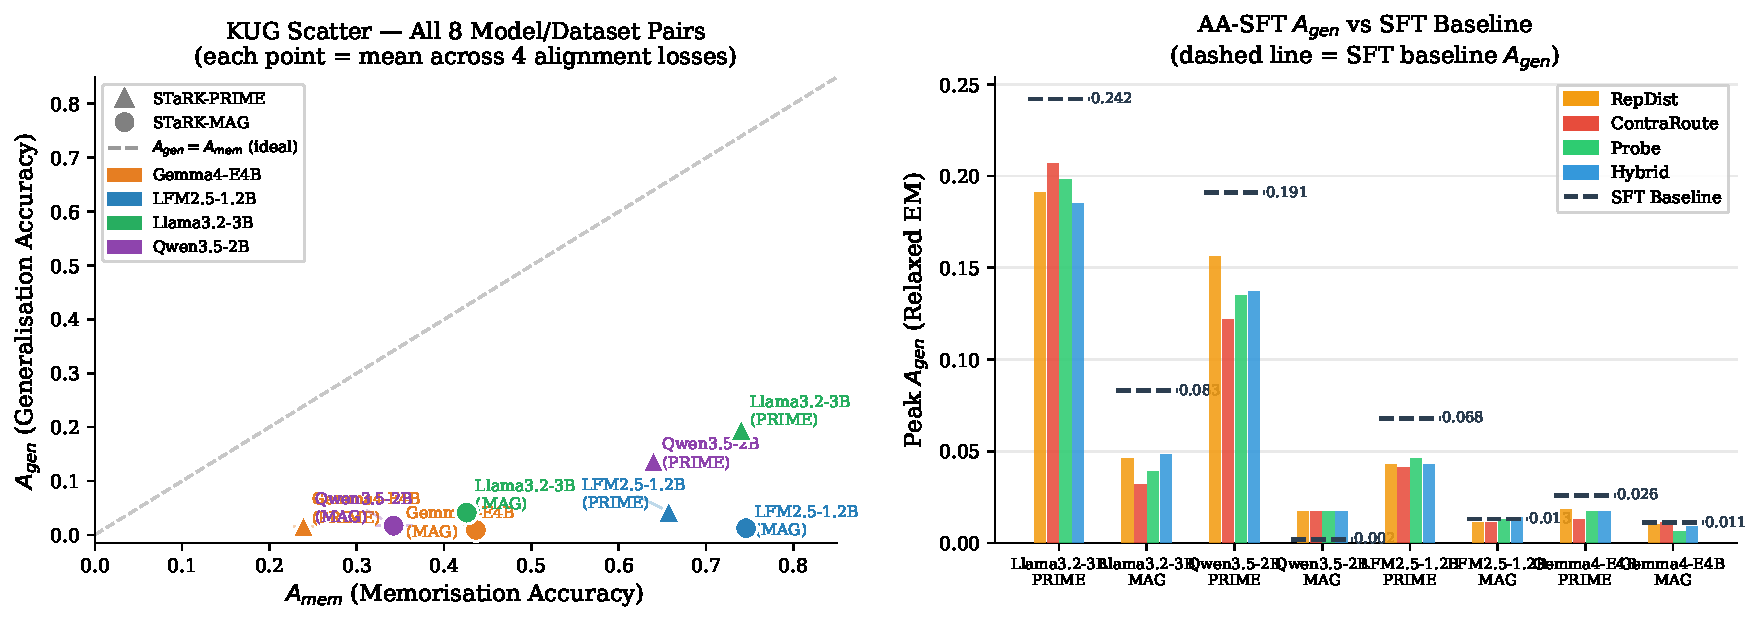
\includegraphics[width=0.48\textwidth]{figures/fig1_kug_scatter.pdf}
  \hfill
  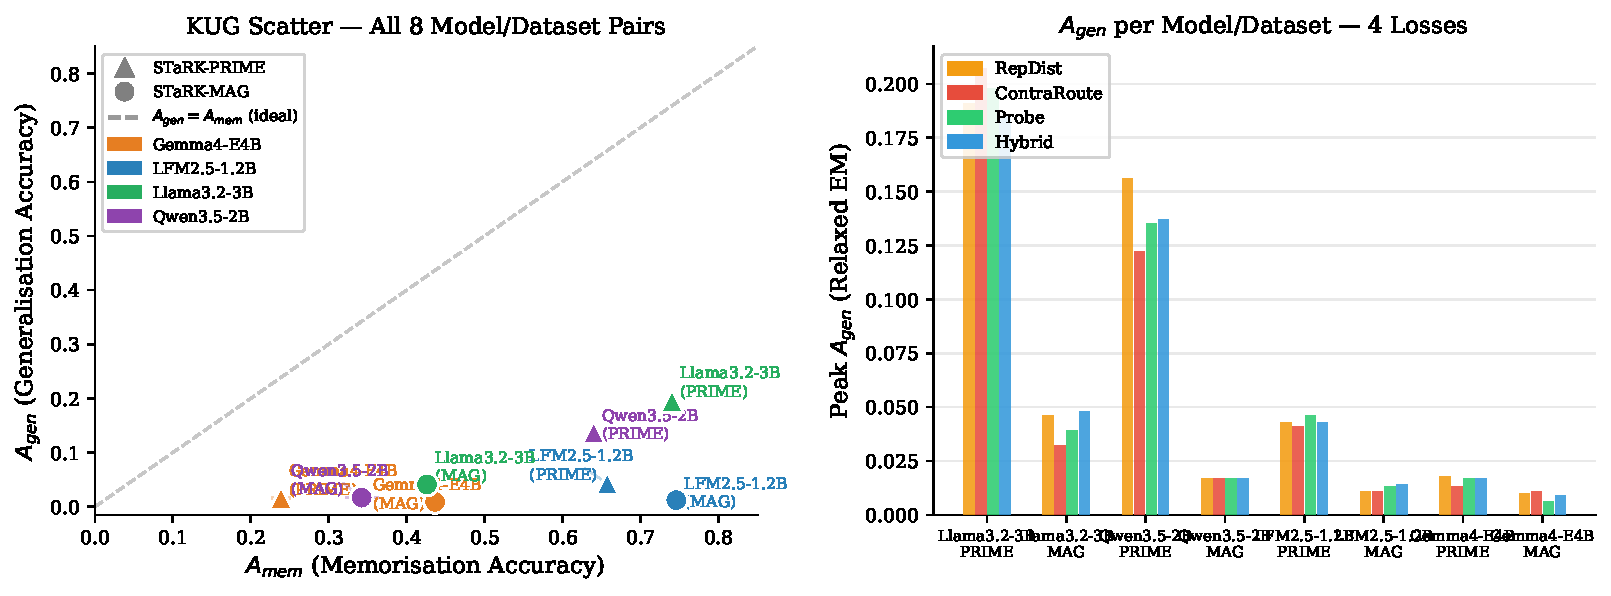
\includegraphics[width=0.48\textwidth]{figures/fig3_v1_gains.pdf}
  \caption{\textbf{Left}: KUG scatter plot. Each point is a (model, dataset) baseline run.
    All points lie below the ideal diagonal ($\Agen=\Amem$), confirming the KUG
    across all 8 runs. STaRK-PRIME points (triangles) cluster higher than STaRK-MAG
    (circles), reflecting the dataset-structure effect.
    \textbf{Right}: Alignment variant peak $\Agen$ per model on both datasets;
    all four losses nearly overlap, confirming loss-function invariance.}
  \label{fig:kug}
  \label{fig:v1gains}
\end{figure*}

\begin{figure}[t]
  \centering
  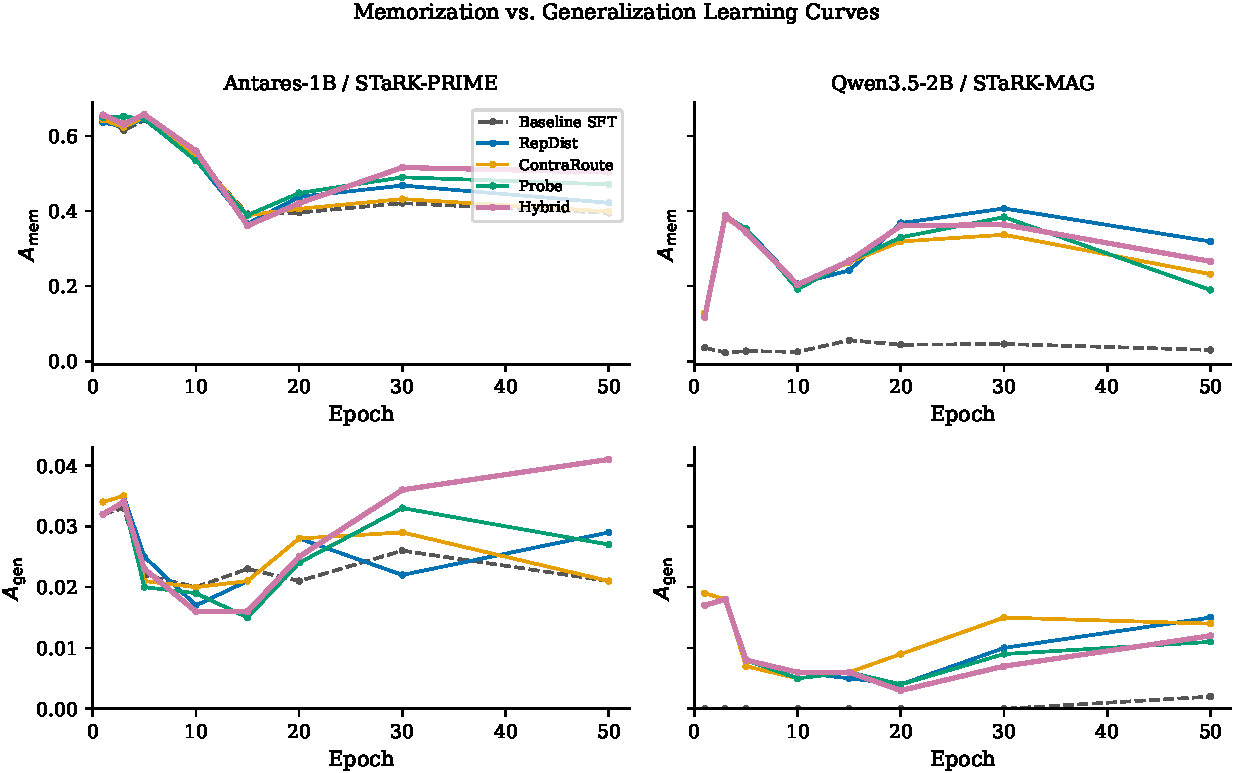
\includegraphics[width=\linewidth]{figures/fig2_learning_curves.pdf}
  \caption{Learning curves for representative model-dataset pairs.
    Top row: $\Amem$ (memorisation, peaks then decays---catastrophic forgetting).
    Bottom row: $\Agen$ (generalisation, stays near zero for baseline; Hybrid lifts it).
    The dual failure pattern visualises the KUG dynamically across training.}
  \label{fig:curves}
\end{figure}

\begin{figure}[t]
  \centering
  \begin{subfigure}[b]{0.48\linewidth}
    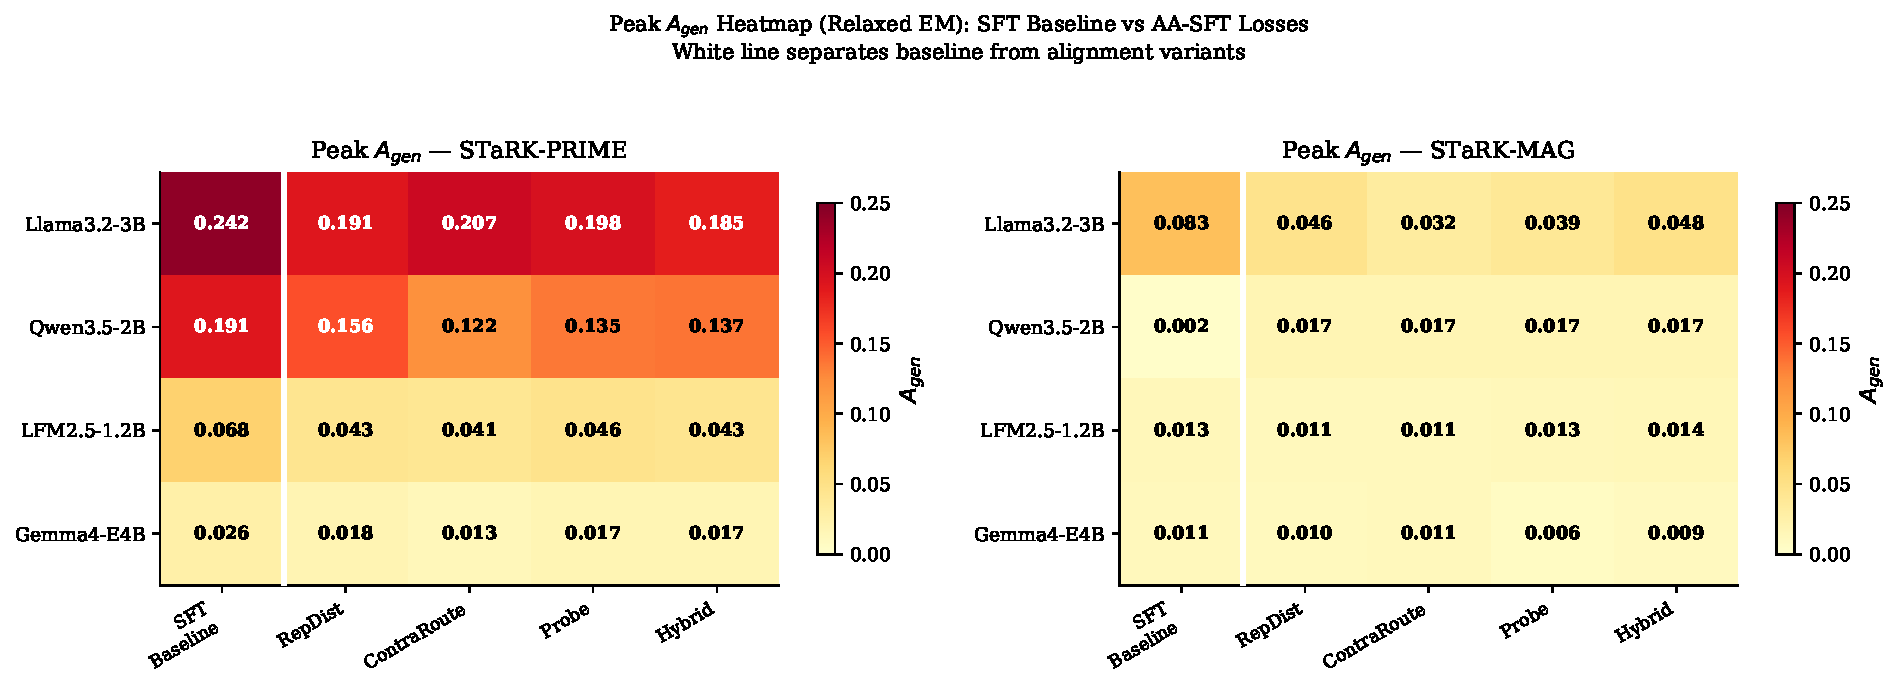
\includegraphics[width=\linewidth]{figures/fig4_v2_vs_v1.pdf}
    \caption{V2 vs.\ V1 relative gains.}
    \label{fig:v2v1}
  \end{subfigure}
  \hfill
  \begin{subfigure}[b]{0.48\linewidth}
    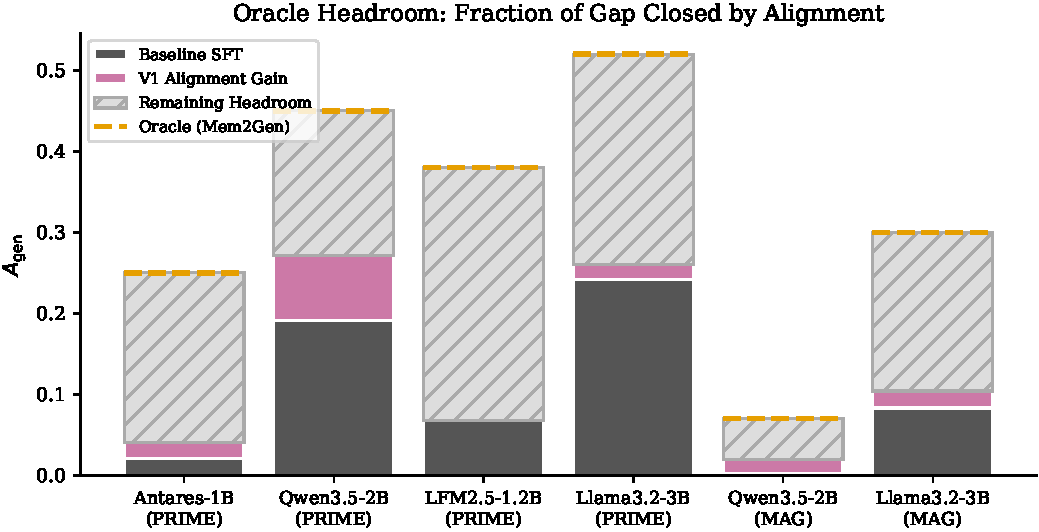
\includegraphics[width=\linewidth]{figures/fig5_oracle_headroom.pdf}
    \caption{Oracle headroom analysis.}
    \label{fig:oracle}
  \end{subfigure}
  \caption{\textbf{Left}: Alignment gains on STaRK-MAG vs.\ STaRK-PRIME across models,
    showing MAG is consistently harder (lower absolute $\Agen$).
    \textbf{Right}: Stacked bars showing baseline $\Amem$, $\Agen$, and remaining headroom
    vs.\ the Mem2Gen oracle. Our best alignment closes $\approx$26--28\% of the oracle gap.}
\end{figure}

%% ═══════════════════════════════════════════════════════════════════════════ %%
% BIBLIOGRAPHY
%% ═══════════════════════════════════════════════════════════════════════════ %%
\bibliography{refs}
\bibliographystyle{acl_natbib}

\end{document}
